\section*{Características demográficas}
En esta sección se hará un análisis de las características demográficas de los usuarios del sistema MiBici. En particular se estudiará la distribución de edades del conjunto de todos los usuarios, la proporción de usuarios por cada género, así como las distribuciones de edades para los usuarios de género masculino y femenino por separado.
\par Al igual que en el resto del reporte, se limitó el estudio de los datos al intervalo de tiempo desde enero del año 2015 hasta diciembre de 2018.
\subsection*{Proporción de usuarios por género}
En total, el número de usuarios diferentes que utilizaron el sistema en el intervalo de enero de 2015 a diciembre 2018 fue $36917$ de los cuales $2$ no registraron su género, $27363$ son de género masculino y $9552$ son de género femenino. Esto puede ser visualizado en la siguiente figura:
\begin{figure}[H]
	\centering
	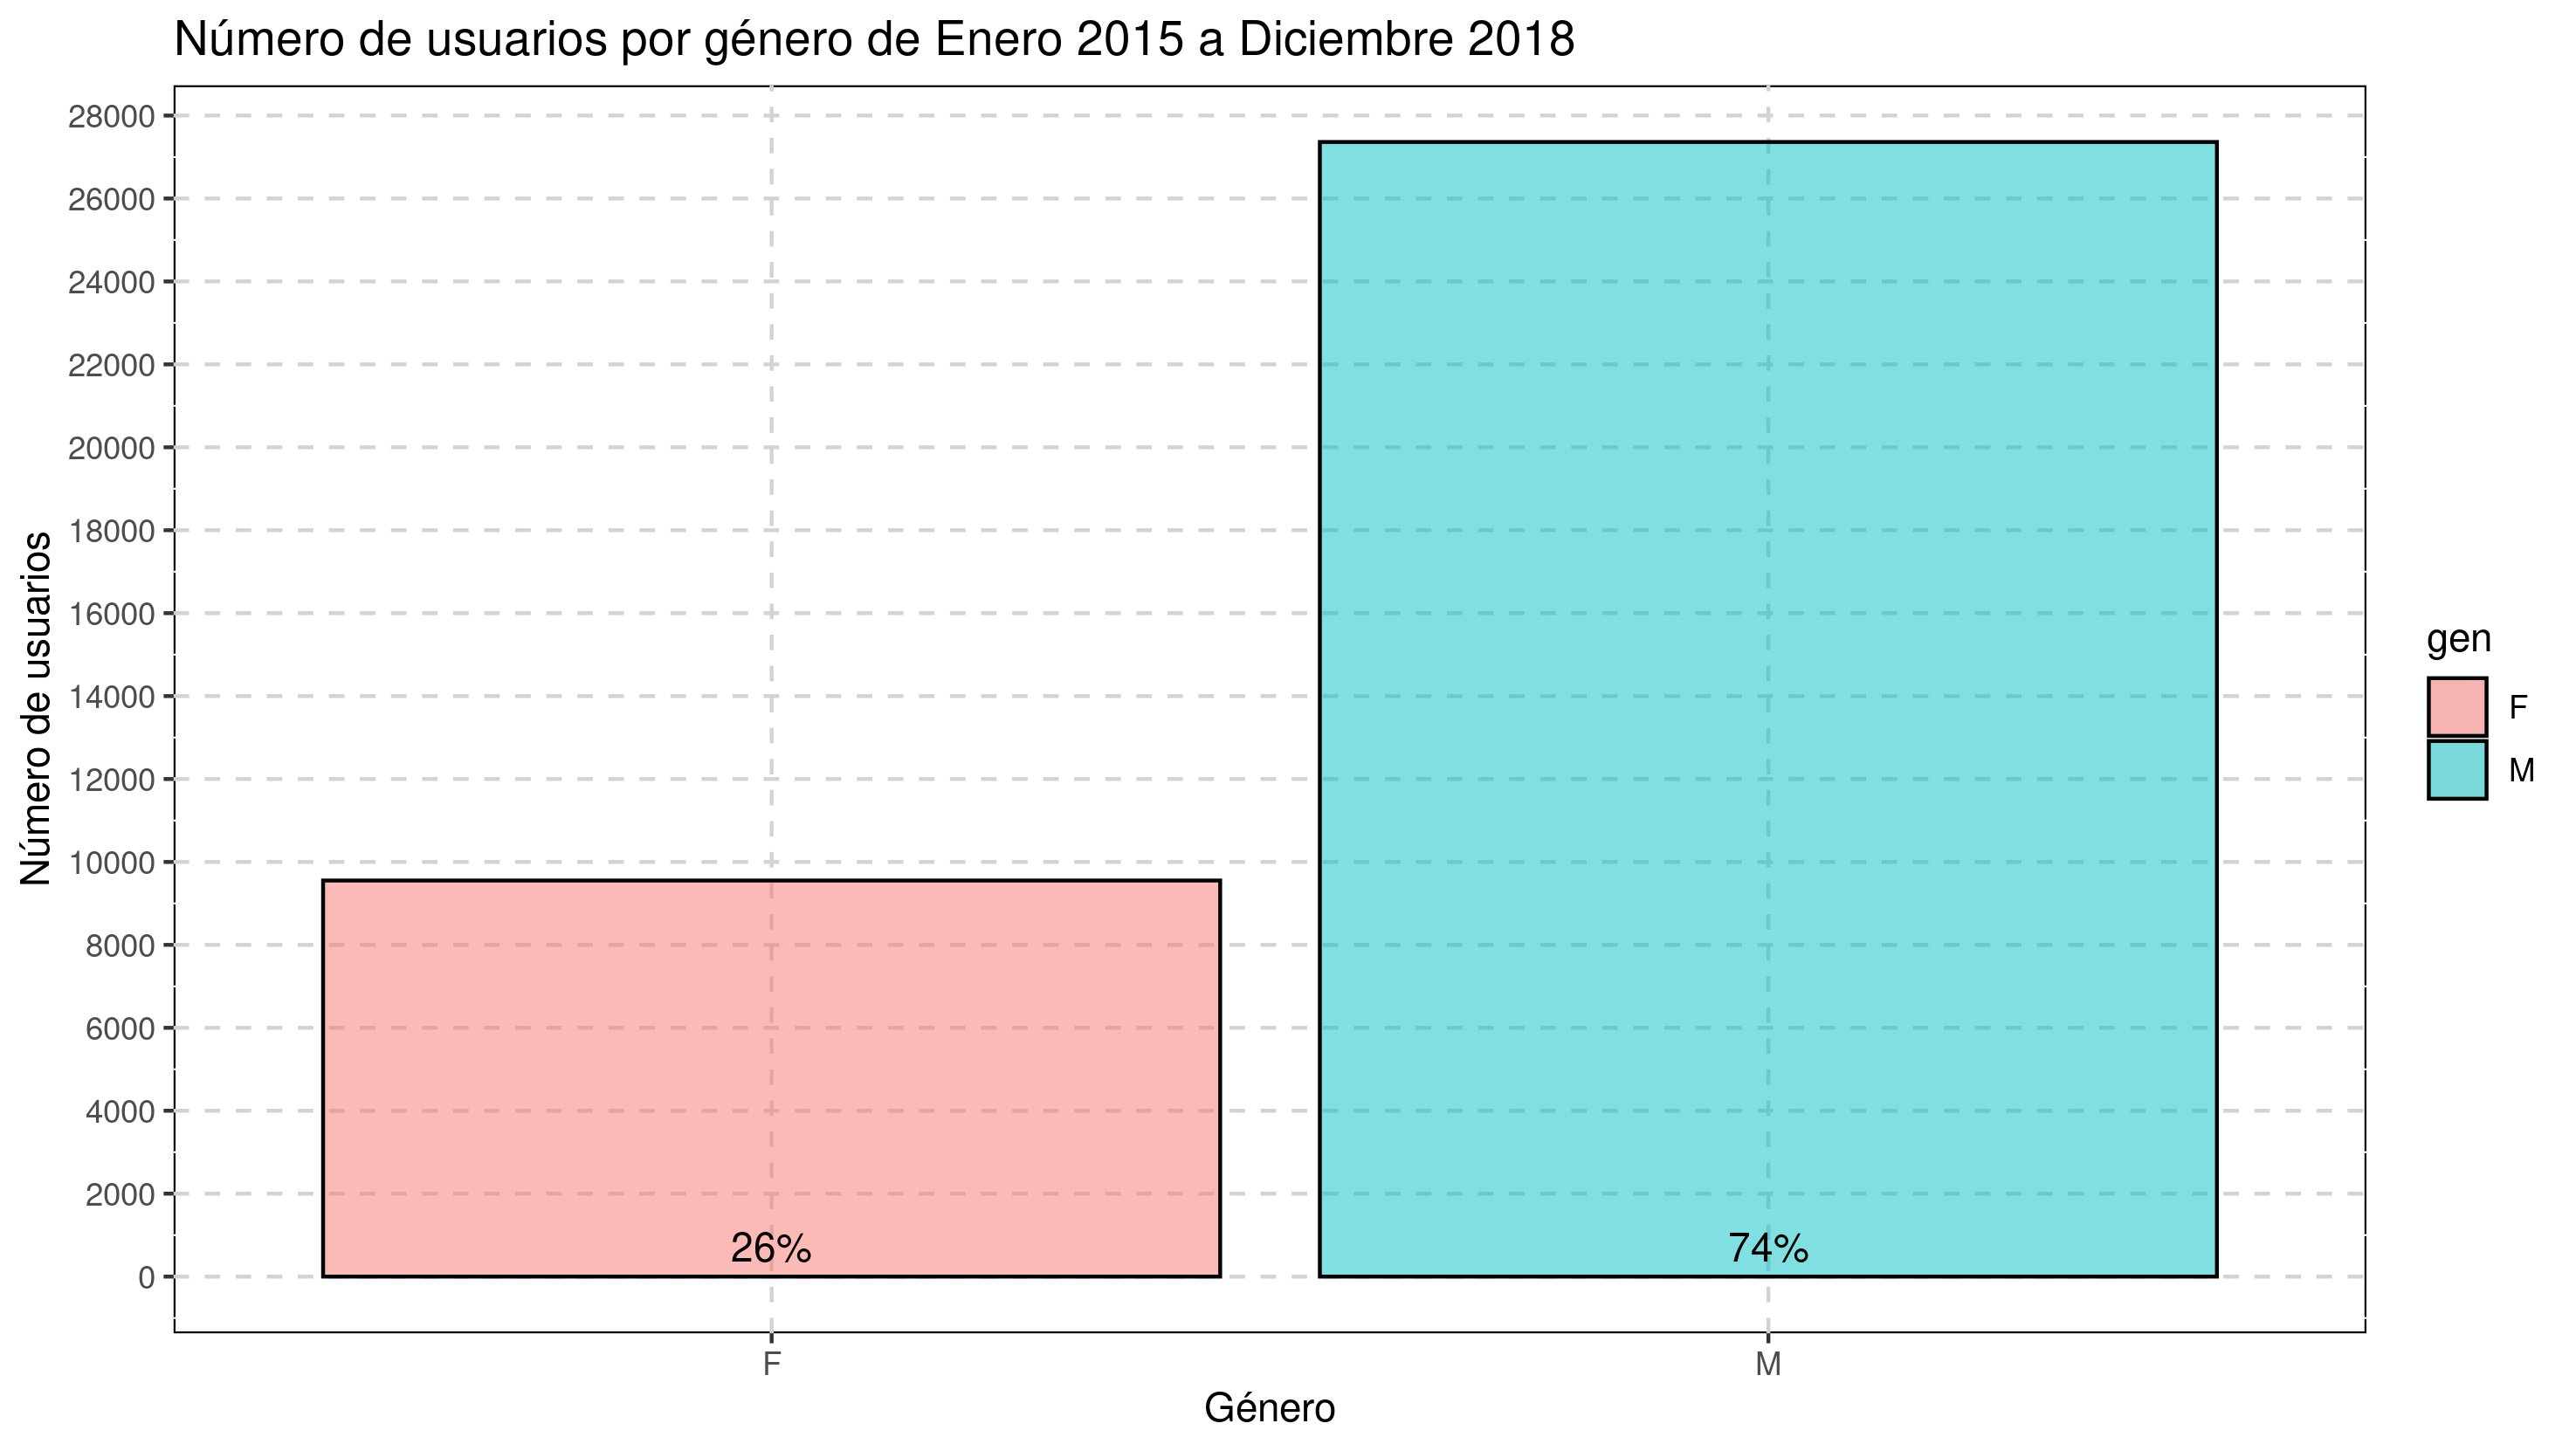
\includegraphics[width=0.7\linewidth]{Graphics/genderProp}
	\caption{Número de usuarios por género de Enero 2015 a Diciembre 2018.}
	\label{fig:genderprop}
\end{figure}
<<<<<<< HEAD
En donde se puede ver que el $74\%$ de los usuarios son hombres y $26\%$ son mujeres. Se deja fuera de la gráfica a los dos usuarios que no registraron su género debido a que su contribución a las proporciones es muy pequeña.
\subsection*{Número de usuarios por edad}
Uno de los requisitos para para poder adquirir una suscripción al sistema MiBici es ser mayor de 16 años, y en caso de ser menor de edad, ser acompañado por un padre o tutor.
=======
En donde se puede ver que el $74\%$ de los usuarios son hombres y $26\%$ son mujeres. Se deja fuera de la gráfica a los dos usuarios que no registraron su género debido a que su contribución a las proporciones es muy pequeña.
>>>>>>> 1e1370b72b0d657fb3209a664d13a4f9856e02f6
